\documentclass{article}
\usepackage{graphicx}
\usepackage[margin=1.5cm]{geometry}
\usepackage{amsmath}

\begin{document}

\title{Tuesday Warm Up: ADCs, and Digital to Analog Converters (DACs)}
\author{Prof. Jordan C. Hanson}

\maketitle

\begin{figure}[ht]
\centering
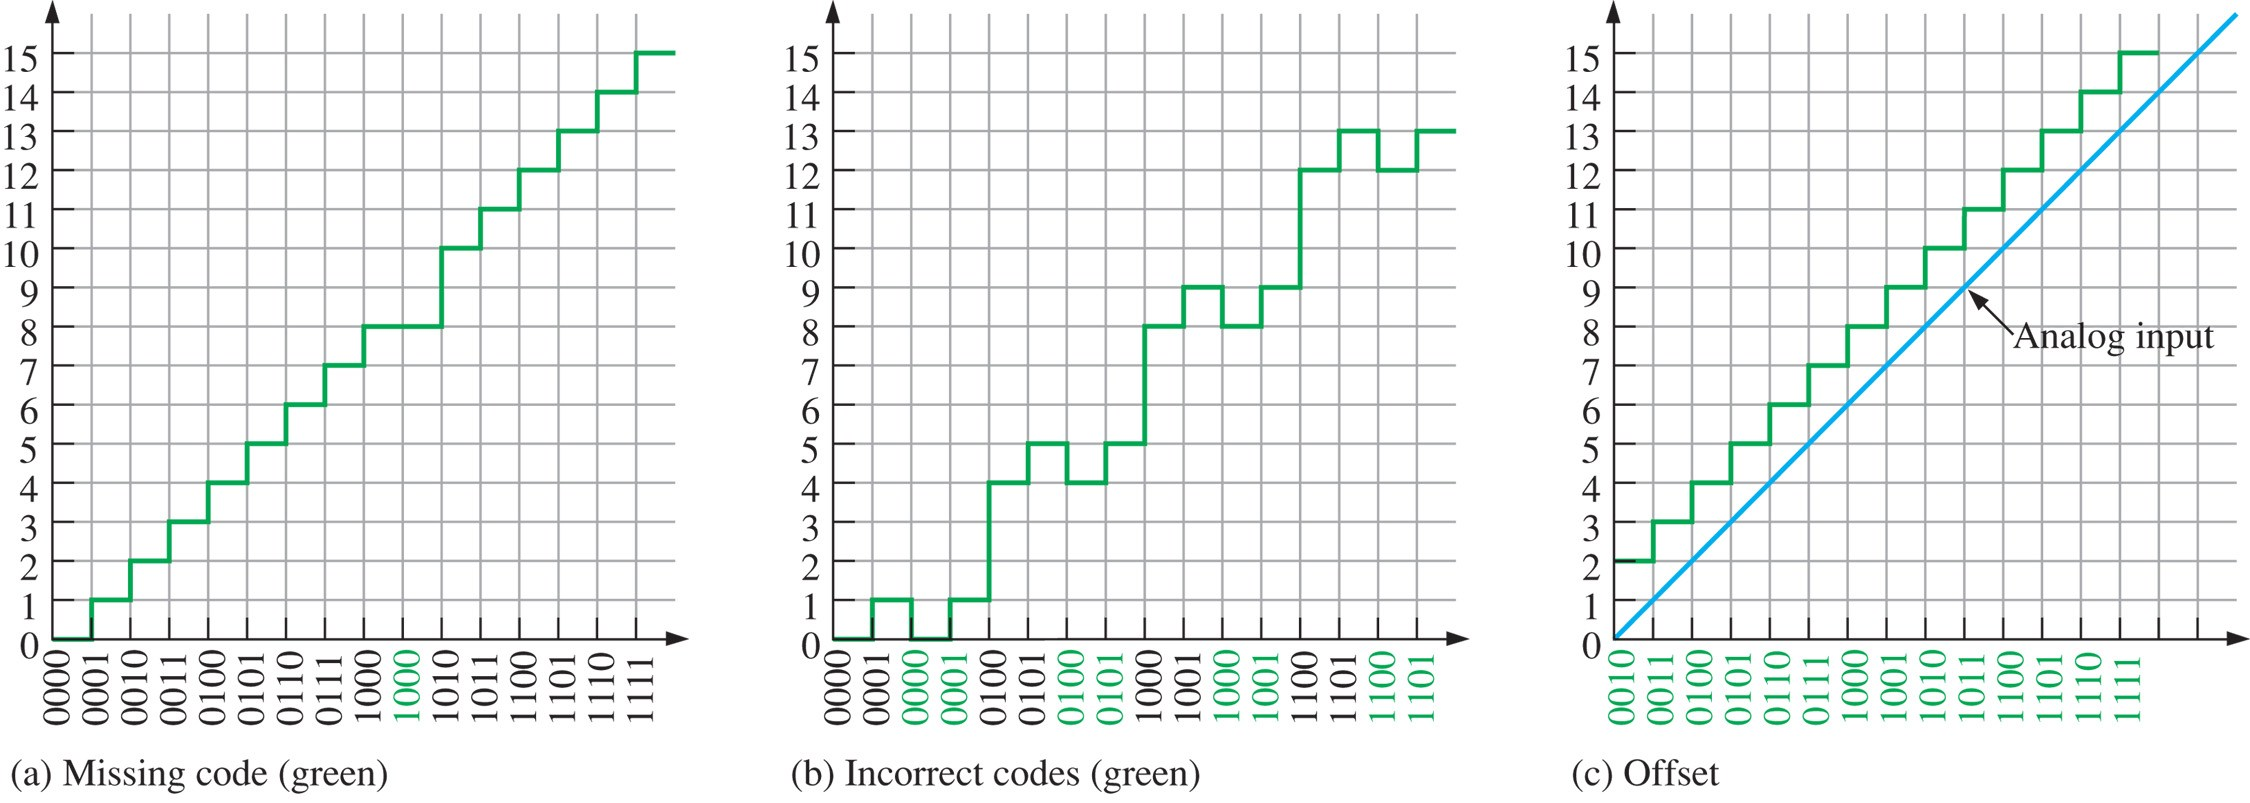
\includegraphics[width=0.75\textwidth]{figures/adc_14.jpg}
\caption{\label{fig:1} Types of ADC errors.}
\end{figure}

\section{Conversion Errors}

\begin{enumerate}
\item (a) Consider Fig. \ref{fig:1} (a).  What analog voltage should go with the ADC output 1000? (b) Consider Fig. \ref{fig:1} (b).  What ADC code should go with the ADC input 15 V? (c) Consider Fig. \ref{fig:1} (c).  What is the binary error that is ocurring relative to the analog voltage input? \\ \vspace{1cm}
\item (a) Consider Fig. \ref{fig:2} (b).  In a DAC, a user inputs 1111, but obtains 11 V instead of 15 V.  What is the voltage error for the code 1001? (b) Consider Fig. \ref{fig:2} (c).  What are the slopes of the three lines, in volts per count?
\end{enumerate}

\begin{figure}[hb]
\centering
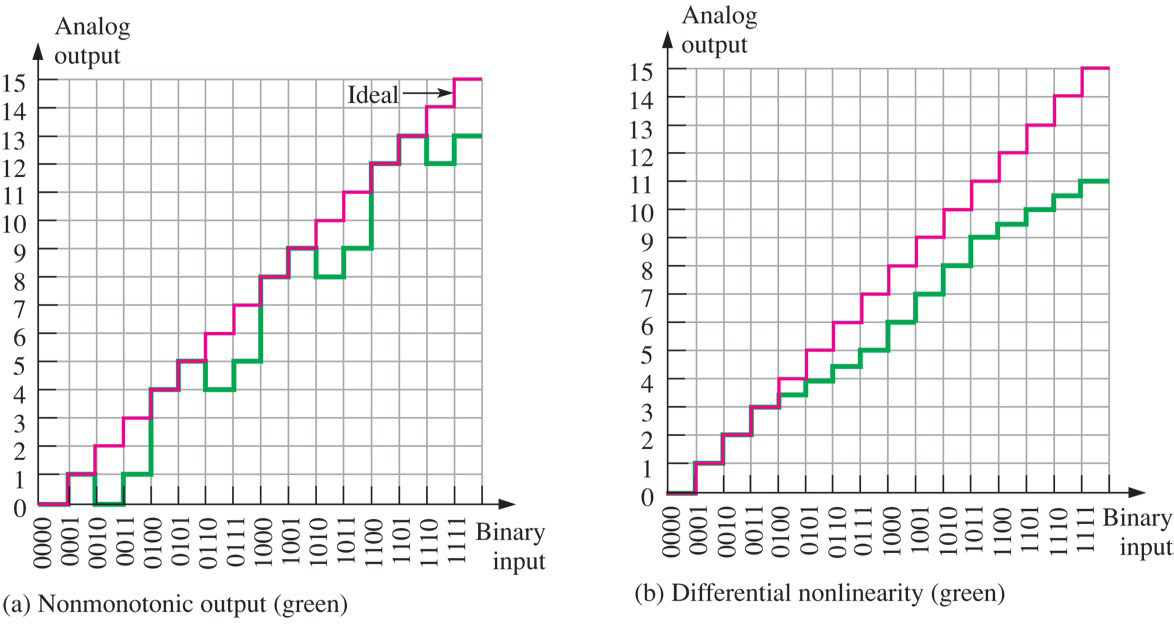
\includegraphics[width=0.49\textwidth]{figures/adc_16.jpg} \hspace{0.1cm}
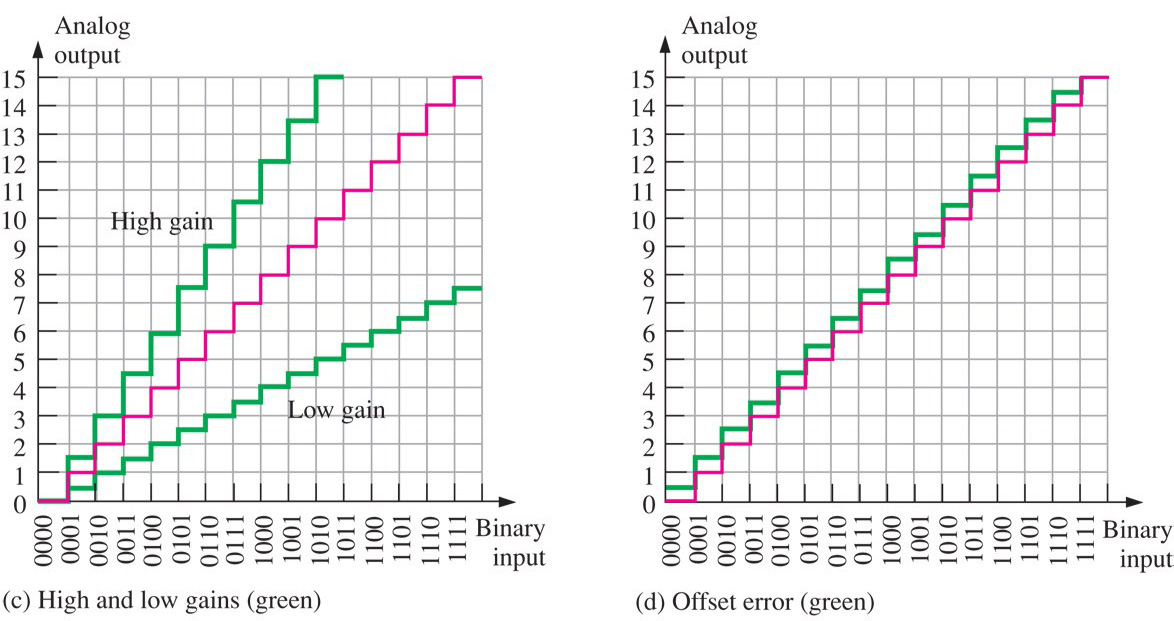
\includegraphics[width=0.49\textwidth]{figures/adc_17.jpg}
\caption{\label{fig:2} (a) DAC coding errors. (b) DAC non-linearity. (c) DAC gain errors. (d) DAC offset errors.}
\end{figure}

\end{document}
